Es werden nach und nach Bauteile des Lock-In-Verstärkers dazugeschaltet
und mithilfe eines Oszilloskops wird das Ausgangssignal abgegriffen. In Abb. \ref{fig:Schema} ist eine schematische Darstellung der einzelnen Bauteile des Lock-In-Verstärkers zu sehen.

\begin{figure}[h]
       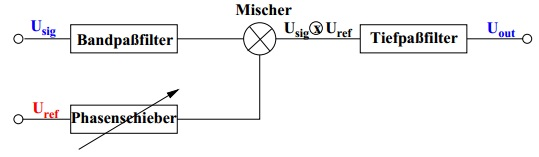
\includegraphics[scale=0.8]{Grafiken/V303Schema.jpg}
       \caption{Aufbau für Signalmessung}
       \label{fig:Schema}
\end{figure}

\subsection{stufenweiser Aufbau}

Als erstes wird ein sinusförmiges Signal mit einer Spannungsamplitude
von \SI{20}{\milli\volt} und einer Frequenz von \SI{1}{\kilo\hertz} erzeugt. (Abb. \cref{fig:AufbauSig1}) Außerdem liefert der Funktionsgenerator ein weiteres Sinussignal, das sog. Referenzsignal, welches durch den Mischer dann multipliziert wird. Eine Abbildung des Referenzsignals ist in Abb. \cref{fig:AufbauSig2} zu sehen. Anschließend wird das zu messende Signal verstärkt. Im nächsten Schritt wird das verstärkte Signal im Mischer mit dem Referenzsignal multipliziert, dabei kommt es je nach Phasenunterschied zu unterschiedlichen Ergebnissen. Hier werden fünf verschiedene Phasen gemessen, welche den Abbildungen \crefrange{fig:Phase1}{fig:Phase5} entsprechen.

Zum Schluss wird das gemischte Signal auf einen Tiefpass gegeben, das durch den Tiefpass gelaufene Signal ist dabei eine Gleichspannung. Für 10 verschiedene Phasen werden die Spannungen am Oszilloskop abgelesen.

\begin{figure}[h]
       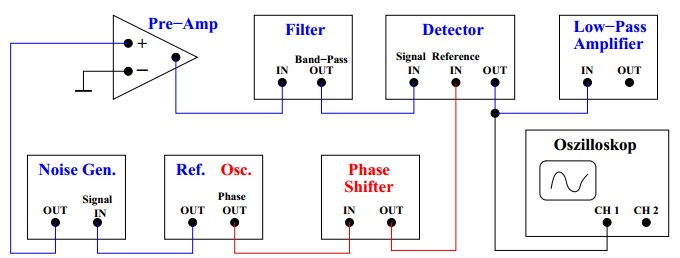
\includegraphics[scale=0.8]{Grafiken/V303Aufbau1.jpg}
       \caption{Aufbau für Signalmessung}
       \label{fig:Aufbau1}
\end{figure}

\subsection{Verrauschtes Signal}

Mit der nun aufgebauten Versuchsanordnung wird nun weiter gearbeitet,
jetzt wird der "noise generator" dazwischen- und eingeschaltet, dabei wird das Sinussignal verrauscht. Der restliche Ablauf unterscheidet sich nicht zu dem im ersten Versuchsteil.

\subsection{Abstandsverhalten der Lichtintensität}

Im letzten Versuchsteil (s. Abb. \ref{fig:Aufbau2})wird die Lichtintensität in Abhängigkeit des Abstandes zur Lichtquelle gemessen wird, es wird gemessen bis kein Signal mehr am Lock-In-Verstärker ablesbar ist. Mit einer Photodiode wird die Lichtintensität gemessen. Dazu werden die in der Leuchtdiode entstehenden Spannungen als Eingangssignal in den Lock-In-Verstärker gegeben. Der Bandpassfilter wird so eingestellt, dass die Amplituden des Signals nach dem Bandpass maximal werden. Der Phasenschieber verschiebt die Phase des Referenzsignals ebenfalls genau so, dass die Amplituden des Ausgangssignals maximal werden. Als Endergebnis erhält man eine Gleichspannung am Ausgang des Lock-In-Verstärkers in Abhängigkeit des Abstandes zwischen Leuchtdiode und Photodiode. Damit auch größere Entfernungen messbar bleiben wird der Faktor, mit dem das Signal verstärkt wird, erhöht. Dies geschieht über den sog. "Gain", welcher später berücksichtigt werden muss.



\begin{figure}[h]
       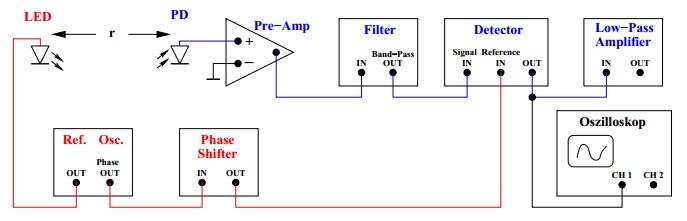
\includegraphics[scale=0.8]{Grafiken/V303Aufbau2.jpg}
       \caption{Aufbau für Abstandsverhalten}
       \label{fig:Aufbau2}
\end{figure}
